\subsection*{Modelización 2}

A día de hoy, la tasa de interés anual sobre la que se remuneran los depósitos en la aplicación Mercado Pago es de un 66\%. Si suponemos un depósito inicial de \$10.000, el dinero crecería en función de la expresión $f(t) = k_0 \cdot (1 + r)^t$, donde $k$ es el capital inicial, en este caso definido como \$10.000; $r$ es la tasa de interés anual, en este ejemplo 0,66; y $t$ sería el tiempo que el dinero tendría que estar depositado en la aplicación. 

Sin embargo, la capitalización no es anual. Para obtener una función más aproximada de la evolución del capital en la aplicación tendríamos que convertir la tasa de interés al período de capitalización, que en este caso es diario tomando un año de 360 días. Por ende, $r = \frac{66}{100} \cdot \frac{1}{360} \approx 0,00183$. La función expresada con capitalización diaria quedaría como:

\begin{align*}
	f(t) &= 10.000 \cdot (1 + 0,00183)^t
\end{align*}

La función independiente en este ejemplo son los días transcurridos. La función dependiente es el capital al final del período.

Se puede representar gráficamente como:

\begin{align*}
	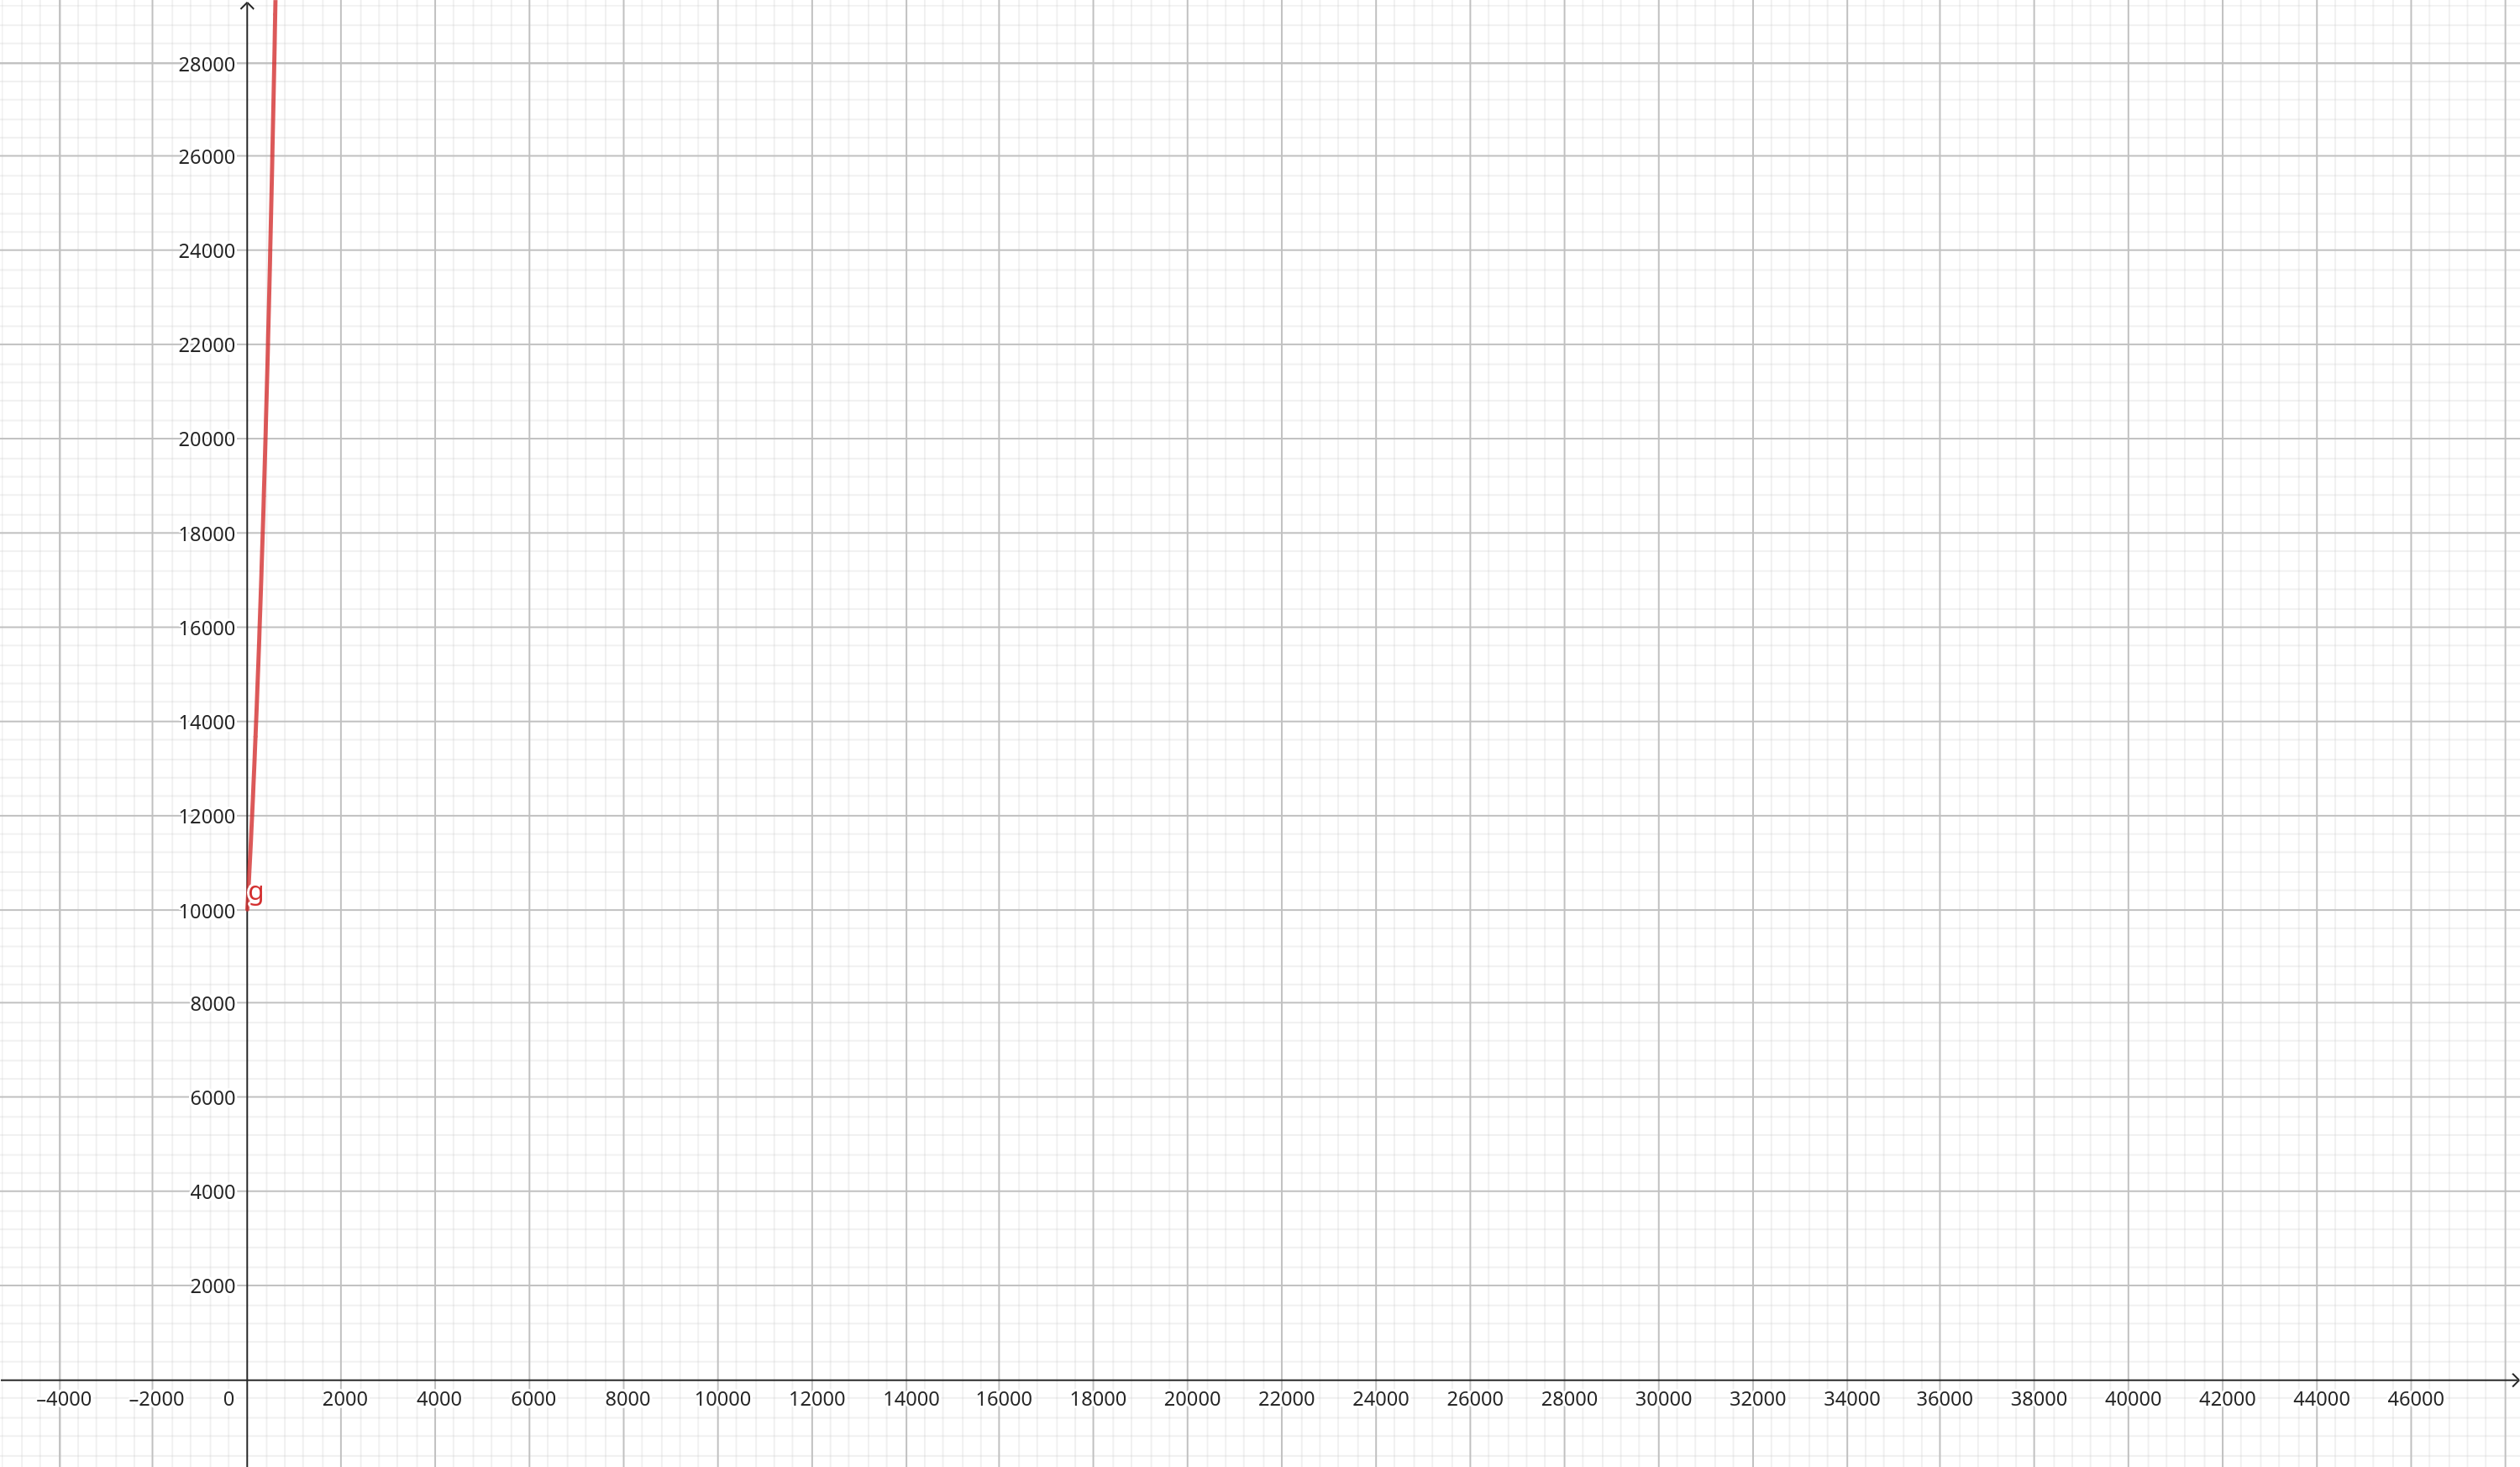
\includegraphics[scale=.15]{02/actividad1/img/modelo2.png}
\end{align*}

Su dominio es $D = [0,+\infty]$ y su conjunto imagen es $I = [10.000, +\infty]$.
